\documentclass[11pt,a4paper]{article}
\usepackage[latin1]{inputenc}
\usepackage{amsmath}
\usepackage{graphicx}
\usepackage{amsfonts}
\usepackage{amssymb}
\title{Practical analysis of very large graphs with the JMaxGraph library}
\author{}
\begin{document}
\maketitle


This article first introduces JMaxGraph, a Java library for the analysis of large graph topologies.

The term "large graph" refers to graph sizes beyond the limit to which usual tools for graph processing can be used.

As an example, the use case we present in this paper uses the graph of Twitter users, which was collected by the DIANA research group (Inria). The dataset comes as a single 215GB text file, in the ADJ format. It stores 
398,846,191 vertices and 23,137,510,395 arcs.
Such a dimensional graph cannot be processed by tools that were not designed with extreme scalability in mind.

JMaxGraph is the result of many years of experience in the development of software tools for graph algorithmics Research within the Coati Research Group at Inria Sophia Antipolis, Universit\'e C\^ote d'Azur, I3S laboratory. JMaxGraph can be seen as a synthesis of these past developements. the Mascopt library started in 2001 aimed at understanding and implementing optimization techniques applied to graphs.
Grph, started in 2008, is a library for the manipulation of large mixed dynamic graphs, was motivated by the limitations of Mascopt in terms of graph models and performance.
The BigGrph project, started in 2014-17,  aimed at improving again the scalability and Grph, was a applied research effort to provide a parallel and 
distributed graph library for the in-memory analysis of large graphs. 
The goal of JMaxGraph is to gather in one comprehensive library the strength of the its ancestor projects, while trying to avoid as much as possible their pitfalls.


\section{State of the Art of graph analysis tools}

Sage, NetworkIt and NetworkX are written in Python. They are highly flexible libraries which are easily usable through the Python interpreter. They compensate the inherent slowness of interpreted Python by offering a facilities and bridges to algorithms written in C. Unfortunately the overhead of frequently switching context between Python and C result in poor performance.

The Boost Graph Library (BGL)
distributed-memory parallelism, you can also look at the Parallel BGL. 

JGraphT and Jung are Java libraries. Their offer a similar Object-oriented model. They both are written in Java, using idiomatic programming paradigm, therefore they both suffer from  the heavy memory model of the JVM. Indeed in the Hotspot JVM, object overhead is 8 bytes and every object occupies a number of bytes that is a multiple of 8. If the number of bytes required by an object for its header and fields is not a multiple 8, then you round up to the next multiple of 8. As a consequence, an instance of a Vertex class with one single int field to store the ID of the vertex  occupies 16 bytes in memory, where it should has only 4 bytes. Each reference to this instance uses 8 more bytes (in a 64bit memory model). Note that if an object is not referenced, it is destroyed by the garbage collector.

The Grph library overcomes this drawback by representing vertices and edges by primitive integers (int values). It accomplishes this by relying on the Fastutil library. 

Hadoop Giraph is a Java distributed graph library build on top of Apache Hadoop. It uses in-memory compression in order to save RAM.
GraphX is a distributed graph library build on top of Spark. It is written in Scale and therefore makes exclusive use of the functional programming paradigm. This feature makes its difficult to non-specialists. GraphX turned out not to scale well because the immutable data model is relies on uses huge amount of memory. Also the results it returns were sometimes wrong.
Both Giraph and GraphX partition the graph across the nodes of computational cluster. The solve the inherent complexity of distributed computing by proposing the BSP programming model. BSP is a vertex-centric message-based programming model which is very adequate to the implementation of simple vertex-centric algorithms. Unfortunately it cannot be used for algorithms that have no natural vertex-centric expression, for which it imposes poor performance because of network congestion due to too numerous messages transiting.
Even vertex-centric algorithm suffer from the distributed nature of the data because the overhead of transiting algorithm local states severely impedes performance.

GraphChi leaves the graph on disk. It proposes an efficient loading mechanism in order to enable on-the-fly processing.

WebGraph is a centralized library written in Java. Its data-structure 
uses compression in order to allow large graphs to fit in RAM. Using this data-structure imposes a compromise between decompression-overhead and compression ratio.

\section{JMaxGraph design}

JMaxGraph benefits from our experience in dealing with existing libraries and in implementing sequential/parallel/distributed graph algorithms.

Its design aims at overcoming the limitations of existing libraries both in terms of scalability and flexiliblity.

Most of existing libraries (JGraphT, Jung, Giraph, WebGraph, GraphX) are designed to run on top of the Java Virtual Machine, so is JMaxGraph. The JVM ensures maximum portability and excellent performance.
It has been developed for more than 20 years by the Sun then Oracle companies which brought it industrial-class quality.

In spite on its intrinsic qualities, Java has a number of limitations. In particular it has intensive RAM usage and method calls overhead when dealing with objects. These entails JMaxGraph
to use and expose a low-level data-structure.

JMaxGraph supports both in-memory (uncompressed) and disk-based (compressed) operations. An algorithm can use both at the same time. Which is required when it needs to operate on both IN and OUT adjacencies but only one one them fits in RAM.
In this case the algorithms must iterate  on the on-disk adjacency while it can access randomly the opposite one.

As of 2018, computational clusters have no node with less that 16 cores. This allows computation to greatly benefit from parellelism.
JMaxGraph then makes extensive use of multi-threading in order to maximum the load of nodes and reduce the overall computation time.

Large experimentation campaigns imply running time which are beyond human's patience. They need to be distributed over the nodes of a cluster. Because of the high probability of failures, their execution needs to be incremental. This enables to recover on error at the point the error occurred. To allow this, JMaxGraph features a custom file-system based Map/Reduce distributed computation engine.

In order to allow this, JMaxGraph has a number of  restriction:



\subsection{Graph model}

In JMaxGraph, vertices are integers. They are implemented by Java primitive int values.

The vertex ID space is contiguous, ranging from 0 to N-1, N being the number of vertices in the graph.

Neighbors are stored in sorted arrays.
This allows $O(log(d(u)))$ search for a given neighbor.

JMaxGraph does not store edges, nor it stores values for edges.

It provides an abstraction for the basic operations than be be performed on adjacencies, regardless of their implementation strategy:
\begin{itemize}
\item $ADJ.getNbVertices()$ : obtaining the number of vertices;
\item $ADJ.iterator(startVertex)$ iterating over the set of vertices, starting at vertex $startVertex$;
\item $ADJ.getNeighbors(u)$ retrieving the neighbors of a given vertex $u$.
\end{itemize}

There currently exist two implementations for adjacencies. One loads dat  in RAM in order to process it efficiently. Another one leaves the data on disk.

An algorithms requiring data to be loaded in RAM can directly use the int array-array, thereby bypassing the OO layer.


\subsection{In-memory data-structure}

Adj-lists are stored in int arrays. Neighbors of vertex $u$ can in found at the $u^{th}$ cell, referred to as $adj[u]$.
Adj-list are ordered. The $u^{th}$ neighbor of vertex $u$ can be obtained by $adj[u][i]$.


JMaxGraph exposes the $int[][]$ to algorithm for the following reason: the graph data can hence be accessed in direct, with no need to do through methods, which woul impose a JMG, passing parameter, thereby manipulation the thread stack. Performance greatly benefits from using this low-level approach.

Java Arrays have another significant advantage: they can be accessed in parallel by threads with no performance loss. Several threads working on distinct areas of an array are then not be slowed done by each other nor they generate inconsistent values.

\subsection{On-disk storage: the JMG data format}


In the JMG format, the graph is described by a directory containing directories for each direction available, IN and/or OUT.

Each of this directory contains at minimum the ARC file for this direction.
ARC files store adjacencies.  An ARC file come with its index file, called \texttt{-index.nbs}, a NBS file being a binary fixed-length encoding for integer numbers.
For each vertex $u$, the index file has an entry which gives the offset in the ARC file at which the set of neighbors of $u$ are stored.

This set of neighbors is encoded at a byte sequence of length:
$$if u < N l = index(u+1) - index(u) else l = size(arcfile) - index(u)$$


Starting at position $index(u)$, the byte sequence encoding the set of neighbors for vertex $u$ is organized like this:
\begin{enumerate}
\item 8 bytes encode the neighbor with lowest ID
\item 1 byte encodes the number of bytes used to store each other neighbor, let us refer to it as $e$. The number of neighbors is then defined by $1 + \frac{l - 9}{e}$.
\item each following neighbor $v_i$ of $u$ is then encoded as the delta $d$ of its ID and the ID of the previous neighbor.
The ID of the $i^{th} (with\ i > 0)$ neighbor is obtained by:
$$v_i = v_{i-1} + d$$.
\end{enumerate}
Since every vertex may use words of different length to store their neighborhood,  the number neighbors cannot be computed out of this $l$.

The JMG file format exhibits the following advantages:
\begin{enumerate}
\item the dataset can be accessed randomly. This means that the degree and the adjacency of any given vertex can be retrieved from disk without having to load/parse other vertices.
\item an ARC file is iterable. This means that adj-list contains in an ARC file can be processed on-the-fly when the file is loaded. This mechanism fastens algorithms which process any adj-list one single time and make it possible to execute certain algorithms even though there is not enough RAM to load the entire graph.
\item there is no vertex in adjacency lists that is not in the vertex set.
\item adjacency lists are compressed in such a way that the more an adj-list is long, the fewer bytes will be used to store each individual element.
\item compression/decompression time is insignificant since it consists in one single addition for every arc.
\end{enumerate}

The Twitter datasets is 3-times smaller when encoded as a JMG datasets rather than stored in an ADJ file.


\subsection{performance of JMG}

The Twitter graph initially came as an ADJ file. The ADJ file format defines that the first line of the file is the number of vertices. Each following line then consists of:
\begin{enumerate}
\item the ID of the vertex;
\item the number of neighbors;
\item the ID for each neighbor.
\end{enumerate}
Numbers are separated by a space.


Using 16MB buffer.
The read throughput of the cluster is 600MB/s. Transferring the entire file to RAM takes 7min.

Using Java standard buffering I/O and number parsing, loading the entire graph takes min. The read throughput then MB/s.

1
2
4
8		4.5=>2.5
16
32

We profiled the execution and we discovered that both  the  basic I/O primitives for reading data from the file and the number parsing methods dramatically slowed down the process. By analyzing the source code of the Java standard library, we found out that the responsible is the excessive number of method calls. These methods had not been in-lined by the just-in-time compiler.

We made a new implementation of buffered reading and number parsing, which speeds up the graph loading process by a factor 30, as illustrated on Figure \ref{fig-a}. Thereby reducing the loading time to 7min. We can see that the graph loading speed is very close to the speed of pure data transfer to memory, which means that the time spent turning text data to graph data-structure is insignificant. Thus at this point, the bottleneck becomes the disk reads. This motivated the definition of a the JMG file format.


\begin{figure}
\begin{center}
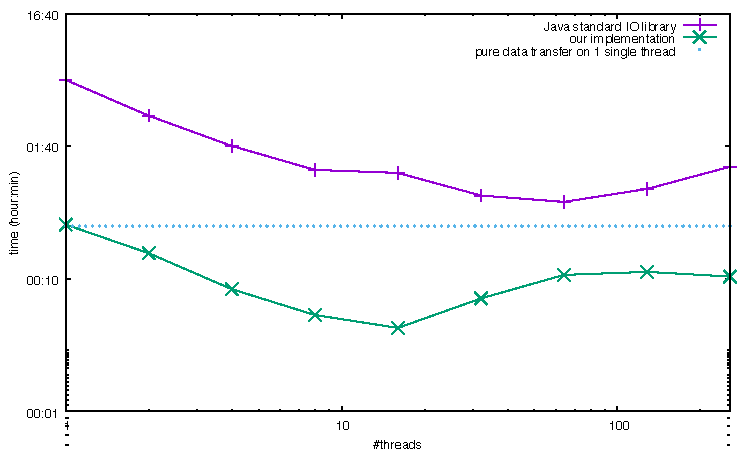
\includegraphics[width=0.8\linewidth]{load.pdf}
\end{center}
\caption{blabla}
\end{figure}





\section{Graph processing models}

This section describes 
graph processing paradigms, and the way it handle each of them.

\subsection{Sequential}

Benefits from direct-access to Java arrays

\subsection{Multi-threaded}

Benefits from concurrent nature of Java arrays.

\subsection{BSP}

JMaxGraph does not support BSP. BSP is useful to distributed computations. In Java, a general model for BSP imposes that messages are objects. Every communication implies instantiating a message object which has too large overhead.

\subsection{Map/Reduce}

When a problem can be divided in a number of sub-problems, it can be solved in parallel on multiple nodes.

JMaxGraph comes with the JMR toolkit, which is a file-based Map/Reduce middleware.

JMR defines that a sub-problem is encoded in a binary file stored in a shared-directory. This relies on shared-filesystem, which is the general rule in today's clusters.

Workers run on various nodes of the clusters. They all have access to the shared directory of not-yet-solved sub-problems, where they pick some.

On completion of a sub-problem, the worker generates a new result files in a shared-directory of results, and it deletes the sub-problem file.

The global computation is assumed to be completed when the sub-problem shared directory is empty.

This has several advantages. There is no need to run distributed data storage servers (like HDFS) because it relies on the cluster shared file-system (NFS, Lustre, etc). Also the system is inherently incremental, which makes it resilient to failures.
Note that they is no restriction whatsoever on the number of workers, which can vary upon time. The most workers, the sooner the computation  will complete.

\section{Algorithms}

\subsection{Counting K2,2 and triangles}

Do we include this?

\subsection{Tarjan}

sequential

optimized

parallel

\subsection{Kernighan-Lin}



\section{Additional features}

\subsection{Progress monitoring}

Algorithms on large datasets often have unknown expected termination date. They will run for a long time, hours days or even months. It is of paramount importance to have information on the running process, in particular an indication of its progress, and a view of its current state (intermediary results).

\end{document}